%%%%%%%%%%%%%%%%%%%%%%%%%%%%%%%%%%%%%%%%%%%%%%%%%%%%%%%%%%%%%%%%%%%%%%%%
%%%  THIS TEX FILE IS TO GENERATE PDF FILE FOR 
%%%     DATA MINING HOMEWORK 04
%%%  COPYRIGHT (C) JIMMY LIN, 2013, UT AUSTIN
%%%%%%%%%%%%%%%%%%%%%%%%%%%%%%%%%%%%%%%%%%%%%%%%%%%%%%%%%%%%%%%%%%%%%%%%
\documentclass[11pt,a4paper]{article}
%%%%%%%%%%%%%%%%%%%%%%%%%%%%%%%%%%%%%%%%%%%%%%%%%%%%%%%%%%%%%%%%%%%%%%%%
%%%  PACKAGES USED IN THIS TEX SOURCE FILE
%%%%%%%%%%%%%%%%%%%%%%%%%%%%%%%%%%%%%%%%%%%%%%%%%%%%%%%%%%%%%%%%%%%%%%%%
\usepackage{geometry,amsthm,amsmath,graphicx,fancyheadings,framed}
\usepackage{tikz}
\usepackage{fancybox}
\usetikzlibrary{automata,positioning}
\usepackage[colorlinks,
            linkcolor=blue,
            anchorcolor=red,
            citecolor=green
            ]{hyperref}
\usepackage[procnames]{listings}
\usepackage{color}
\usepackage{/Users/JimmyLin/workspace/latexTemplate/UTA_CS/JS}
\usepackage{/Users/JimmyLin/workspace/latexTemplate/UTA_CS/JSASGN}
%%%%%%%%%%%%%%%%%%%%%%%%%%%%%%%%%%%%%%%%%%%%%%%%%%%%%%%%%%%%%%%%%%%%%%%%
%%% MACROS CONTAINING THE FILE INFORMATION
%%%%%%%%%%%%%%%%%%%%%%%%%%%%%%%%%%%%%%%%%%%%%%%%%%%%%%%%%%%%%%%%%%%%%%%%
\renewcommand{\COURSE}{CS363D Statistical Learning and Data Mining}
\renewcommand{\LECTURER}{Pradeep Ravikumar}
\renewcommand{\TUTOR}{Adarsh Prasad}
\renewcommand{\TASK}{Homework 05}
\renewcommand{\RELEASEDATE}{April. 21 2014}
\renewcommand{\DUEDATE}{April. 28 2014}
\renewcommand{\TIMECONSUME}{7 hours}
%%%%%%%%%%%%%%%%%%%%%%%%%%%%%%%%%%%%%%%%%%%%%%%%%%%%%%%%%%%%%%%%%%%%%%%%
%%% DOCUMENTATION STARTS FROM HERE 
%%%%%%%%%%%%%%%%%%%%%%%%%%%%%%%%%%%%%%%%%%%%%%%%%%%%%%%%%%%%%%%%%%%%%%%%
\begin{document}
%%%%%%%%%%%%%%%%%%%%%%%%%%%%%%%%%%%%%%%%%%%%%%%%%%%%%%%%%%%%%%%%%%%%%%%%
%% TITLE PAGE
%%%%%%%%%%%%%%%%%%%%%%%%%%%%%%%%%%%%%%%%%%%%%%%%%%%%%%%%%%%%%%%%%%%%%%%%
\begin{titlepage}
    \maketitle
\end{titlepage}
%%%%%%%%%%%%%%%%%%%%%%%%%%%%%%%%%%%%%%%%%%%%%%%%%%%%%%%%%%%%%%%%%%%%%%%%
%% CONTENT PAGE: TABLEOFCONTENTS, LISTOFTABLES, LIST OF FIGURES
%%%%%%%%%%%%%%%%%%%%%%%%%%%%%%%%%%%%%%%%%%%%%%%%%%%%%%%%%%%%%%%%%%%%%%%%
\renewcommand{\contentsname}{Contents}
\begin{center} 
    \tableofcontents 
    %\listoftables 
    \listoffigures
\end{center}
\newpage
%%%%%%%%%%%%%%%%%%%%%%%%%%%%%%%%%%%%%%%%%%%%%%%%%%%%%%%%%%%%%%%%%%%%%%%%
%%% GENERAL DOCUMENTATION BEGINS 
%%%%%%%%%%%%%%%%%%%%%%%%%%%%%%%%%%%%%%%%%%%%%%%%%%%%%%%%%%%%%%%%%%%%%%%%
\section{Short Answer Question}

\subsection{superset}
(a) Can a superset of an infrequent itemset be frequent? Why or why not?

Of course not. This is because the support of superset is always lower than or
equals to the support of that infrequent itemset itself. (the total number of
transactions are fixed and the support count of superset is always lower
than or equals to the support count of that infrequent itemset itself.)

\subsection{confidence}
(b) Let x denote an item that occurs in every transaction of a dataset. What
can you say about the confidence of a rule of the form $y \rightarrow x$, where y is
some item in the dataset that appears in at least one transaction?

According to the given condition, we can see the support count 
\begin{align}
    \sigma(y,x) &= \sigma(y) \\
    \sigma(x) &= |T|
\end{align}

The confidence related to that rule $y \rightarrow x$ is

\begin{align}
    c(y \rightarrow x) = \frac{\sigma(y,x)}{\sigma(y)} = 1
\end{align}

Hence, the confidence of $y \rightarrow x$ is $1$.

\subsection{threshold} 
(c) Let $Y$ denote a frequent itemset. We are interested in generating rules
from $Y$ that have a confidence of at least $c$. Let $X \rightarrow Y - X$ be a rule
that does not satisfy the confidence threshold. Let $X′ \subseteq X$. Can 
$X′ \rightarrow Y - X′$ satisfy the confidence threshold? Give reasons.

According to the known condition, 

\begin{align}
    c(X \rightarrow Y - X) = \frac{\sigma(Y)}{\sigma(X)} < minconf
\end{align}

Since the $X'$s is the subset of $X$, we have

\begin{align}
    \sigma(X') \geq \sigma(X)
\end{align}

We get the relationship between 
\begin{align}
    c(X′ \rightarrow Y - X′) = \frac{\sigma(Y)}{\sigma(X')} \leq
    \frac{\sigma(Y)}{\sigma(X)} < minconf
\end{align}

Hence, it can be concluded that 

\begin{align}
    c(X′ \rightarrow Y - X′) \text{ does not satisfy the confidence threshold.}
\end{align}

\newpage
\section{Apriori algorithm}
\subsection{Lattice}
(a) Draw an itemset lattice representing the dataset given in Table 1.

\begin{figure}[h]
    \centering
    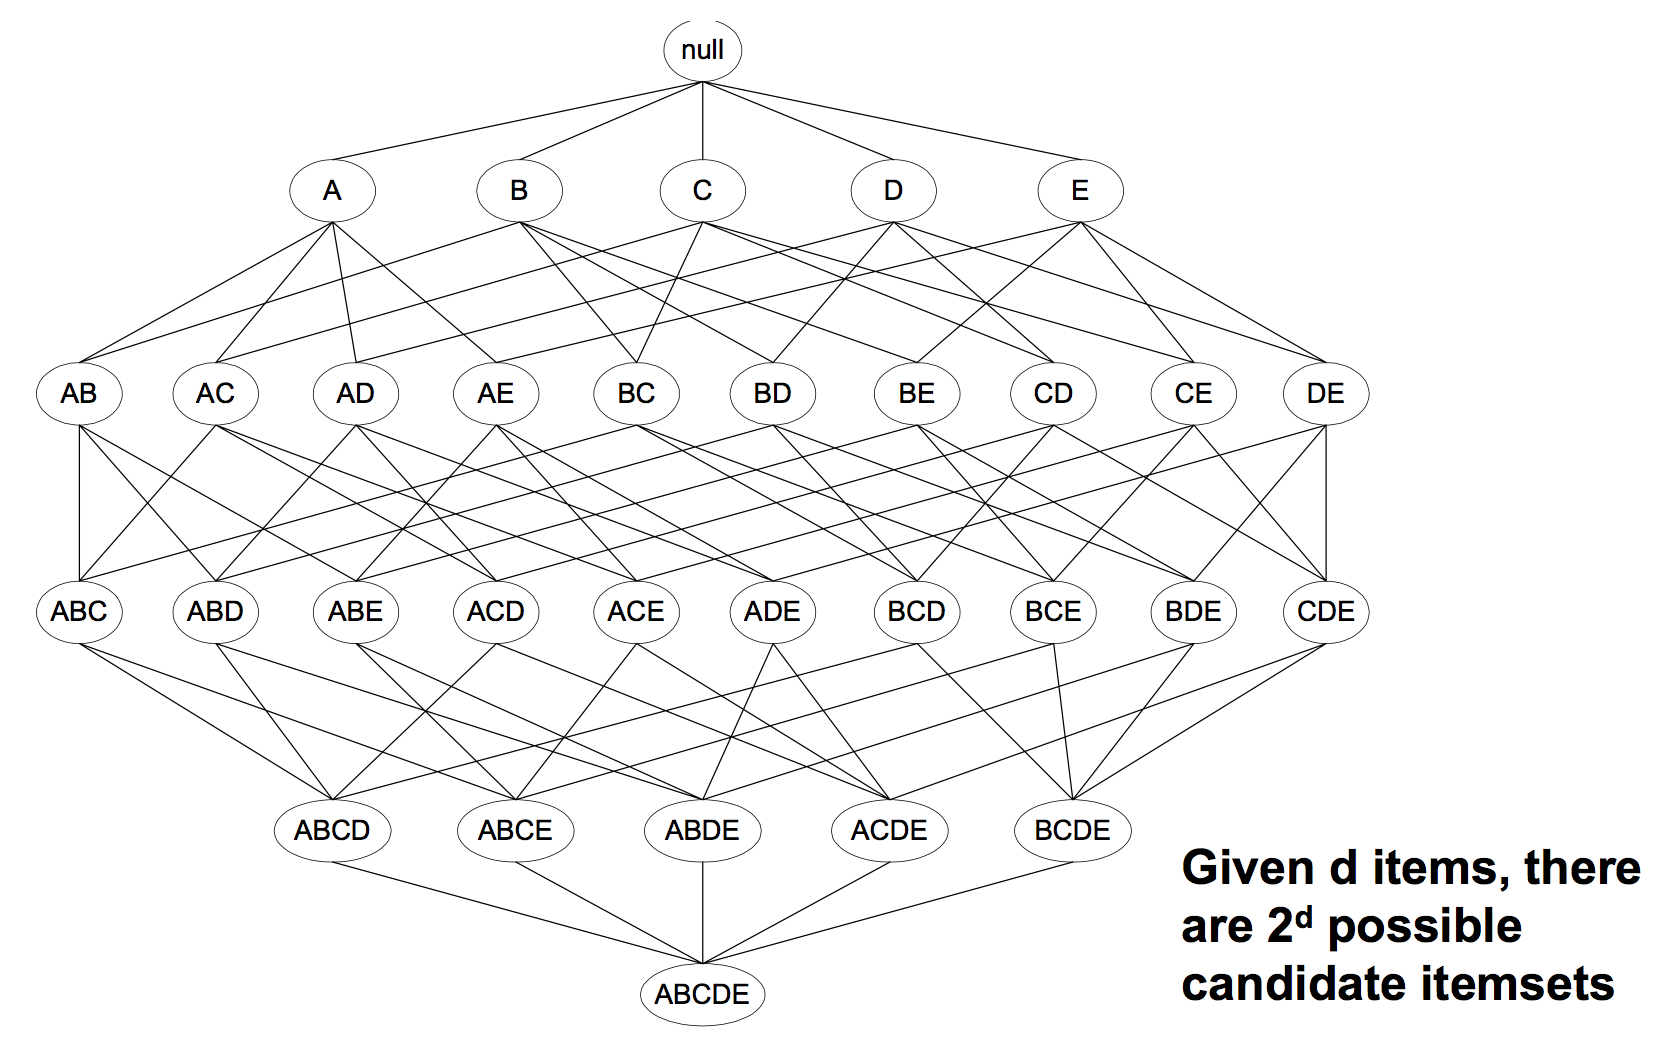
\includegraphics[width=6.5in,height=4.5in]{./lattice.png}
    \caption{Itemset Lattice (Refer to the Class Note)}
\end{figure}

Note that the representation of itemsets in the lattice is corresponding to
lower-cased items in our setting.

\subsection{Frequent Itemsets}
(b) What is the percentage of frequent itemsets (with respect to all itemsets
in the lattice)?

The total number of nodes in the lattice is $|T| = 2^{5} = 32$.

The number of frequent itemsets is $16$.

The percentage of frequent itemsets is $\frac{16}{32} = \frac{1}{2}$.

\subsection{Candidate Itemsets}
(c) What is the percentage of candidate itemsets that are found to be
infrequent after support counting?

The total number of nodes in the lattice is $|T| = 2^{5} = 32$.


Candidate itemsets that found to be infrequent after support counting are ac,
ce, abd, abe, bcd, abde. 

The percentage of infrequent itemsets is $\frac{6}{32} = \frac{3}{16}$

\newpage
\appendix
\section{Codes to count frequency}
\definecolor{keywords}{RGB}{0,0,0}
\definecolor{comments}{RGB}{0,0,0}
\definecolor{red}{RGB}{0,0,0}
\definecolor{green}{RGB}{0,0,0}
\lstset{language=Python, 
        basicstyle=\ttfamily\small, 
        keywordstyle=\color{keywords},
        commentstyle=\color{comments},
        stringstyle=\color{red},
        showstringspaces=false,
        identifierstyle=\color{green},
        procnamekeys={def,class}}
\lstinputlisting[language=Python]{./count.py}

\newpage
\section{Result Demo of Codes}
\lstinputlisting{./result.txt}
%%%%%%%%%%%%%%%%%%%%%%%%%%%%%%%%%%%%%%%%%%%%%%%%%%%%%%%%%%%%%%%%%%%%%%%%
%%% General Documentation ends
%%%%%%%%%%%%%%%%%%%%%%%%%%%%%%%%%%%%%%%%%%%%%%%%%%%%%%%%%%%%%%%%%%%%%%%%
\end{document}
